\documentclass[12pt]{article}
\usepackage[margin=1in]{geometry} 
\usepackage{graphicx}
\usepackage{amsmath,amsthm,amssymb}
\usepackage{hyperref}
\usepackage{tikz}

\title{
    \textbf{Theory Assignment 2} \\ 
    \textbf{CS5280} \\
}

\author{
    \textbf{Darpan Gaur} \\
    \textbf{CO21BTECH11004}
}


\date{}

\begin{document}
\maketitle

\hrulefill

\section*{Problem 1}
\begin{equation*}
    s = r_1(x) r_3(x) w_3(y) w_2(x) r_4(y) c_2 w_4(x) c_4 r_5(x) c_3 w_5(z) c_5 w_1(z) c_1
\end{equation*}
% FSR-> $t_5 t_3 t_1 t_2 t_4$\\
\textbf{FSR} \\
For a history $s \in \text{FSR}$, there exists a serial history $s'$ such that LRF($s$) = LRF($s'$).\\
Consider $s' = t_5 t_3 t_1 t_2 t_4$. Hence, $s' = r_5(x) w_5(z) r_3(x) w_3(y) r_1(x) w_1(x) w_2(x) r_4(y) w_4(x) c_5 c_3 c_1 c_2 c_4 $.\\
\begin{equation*}
    \begin{aligned}
        \text{LRF}(s) &= \{(t_0, x, t_1), (t_0, x, t_3), (t_3, y, t_4) , (t_4, x, t_\infty), (t_3, y, t_\infty), (t_1 , z, t_\infty) \} \\
        \text{LRF}(s') &= \{(t_0, x, t_3), (t_0, x, t_1), (t_3, y, t_4), (t_4, x, t_\infty), (t_3, y, t_\infty), (t_1 , z, t_\infty) \}
    \end{aligned}
\end{equation*}
As LRF($s$) = LRF($s'$), hence $s \in \text{FSR}$.\\
\\
\textbf{VSR} \\
For a history $s \in \text{VSR}$, there exists a serial history $s'$ such that RF($s$) = RF($s'$).\\
\begin{equation*}
    \text{RF}(s) = \{(t_0, x, t_1), (t_0, x, t_3), (t_3, y, t_4), (t_4, x, t_5), (t_4, x, t_\infty), (t_3, y, t_\infty), (t_1, z, t_\infty) \}
\end{equation*}
Proof by contradiction. \\
Let us assume that $s \in \text{VSR}$. So there exists a serial history $s'$ such that RF($s$) = RF($s'$).\\
In RF($s$): -
\begin{itemize}
    \item $(t_4, x, t_5)$, so $t_4$ preceeds $t_5$ in $s'$, i.e., $t_4 < t_5$.
    \item $(t_3, y, t_4)$, so $t_3$ preceeds $t_4$ in $s'$, i.e., $t_3 < t_4$.
    \item $(t_1, z, t_\infty)$, and both $t_1$ and $t_5$ have $w(z)$ operations, so $t_5 preceeds t_1$ in $s'$, i.e., $t_5 < t_1$.
    \item $(t_0, x, t_3), and (t_0, x, t_1)$, so $t_1$ and $t_3$ preceeds $w_2(x)$ hence $t_2$ in $s'$, i.e., $t_1 < t_2$ and $t_3 < t_2$.
\end{itemize} 
From above restrictinos we get the following order for $s'$: $t_3 < t_4 < t_5 < t_1 < t_2$. \\
But this is not possible as $t_2$ at end in $s'$ will change $(t_4, x, t_\infty)$ to $(t_2, x, t_\infty)$, which is not in RF($s$). Hence contradiction, and $s \notin \text{VSR}$.\\
\\
\textbf{CSR} \\
% CSR-> Conflict graph cyclic\\ 
For a history $s \in \text{CSR}$, we need to show that the conflict graph of $s$ is acyclic.\\
Conflict graph is shown in Figure \ref{fig:conflict_graph_q1}.\\
As there exist a cycle $t_1 \rightarrow t_2 \rightarrow t_4 \rightarrow t_5 \rightarrow t_1$, therefore conflict graph is cyclic and $s \notin \text{CSR}$.
\begin{figure*}[h]
    \centering
    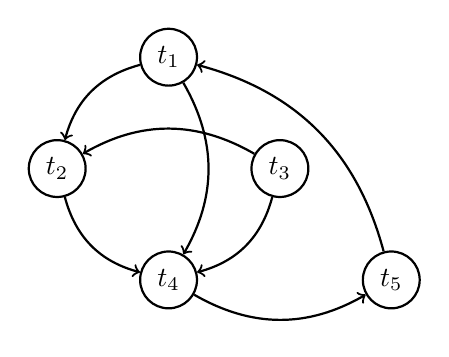
\begin{tikzpicture}[node distance={2cm}, thick, main/.style = {draw, circle}]
        \node[main] (1) {$t_1$};
        \node[main] (2) [below left of=1] {$t_2$};
        \node[main] (3) [below right of=1] {$t_3$};
        \node[main] (4) [below right of=2] {$t_4$};
        \node[main] (5) [below right of=3] {$t_5$};

        \path[->] (1) edge [bend right] node {} (2);
        \path[->] (1) edge [bend left] node {} (4);
        
        \path[->] (3) edge [bend right] node {} (2);
        \path[->] (3) edge [bend left] node {} (4);

        \path[->] (2) edge [bend right] node {} (4);

        \path[->] (4) edge [bend right] node {} (5);    

        \path[->] (5) edge [bend right] node {} (1);
        
    \end{tikzpicture}
    \caption{Conflict Graph}
    \label{fig:conflict_graph_q1}
\end{figure*}


\section*{Problem 2}
\begin{equation*}
    s = r_1(z) r_3(x) r_2(z) w_1(z) w_1(y) c_1 w_2(y) w_2(u) c_2 w_3(y) c_3
\end{equation*}
\textbf{VSR} \\
We know that history $s$ is view serializable if there exists a serial history $s'$ such that RF($s$) = RF($s'$).
Consider $s' = t_2 t_1 t_3$. Hence, $s' = r_2(z) w_2(y) w_2(u) r_1(z) w_1(z) w_1(y) r_3(x) w_3(y) c_1 c_2 c_3$.\\
\begin{equation*}
    \begin{aligned}
        \text{RF}(s) &= \{(t_0, z, t_1), (t_0, x, t_3), (t_0, z, t_2), (t_0, x, t_\infty), (t_3, y, t_\infty), (t_2, u, t_\infty), (t_0, z, t_\infty) \} \\
        \text{RF}(s') &= \{(t_0, z, t_2), (t_0, z, t_1), (t_0, x, t_3), (t_0, x, t_\infty), (t_3, y, t_\infty), (t_2, u, t_\infty), (t_0, z, t_\infty) \}
    \end{aligned}
\end{equation*}
As op($s$) = op($s'$) and RF($s$) = RF($s'$), hence $s$ is view serializable.\\
\\
\textbf{CSR} \\
Conflict graph is shown in Figure \ref{fig:conflict_graph_q2}.\\ As the conflict graph of $s$ is cyclic, $ s \notin \text{CSR}$.
\begin{figure*}[h]
    \centering
    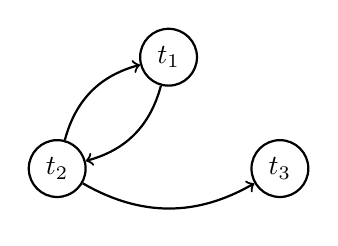
\begin{tikzpicture}[node distance={2cm}, thick, main/.style = {draw, circle}] 
        \node[main] (1) {$t_1$};
        \node[main] (2) [below left of=1] {$t_2$};
        \node[main] (3) [below right of=1] {$t_3$};

        % \draw[->] (2) -- (1);
        % \draw[->] (1) -- (2); 
        \path[->] (1) edge [bend left] node {} (2);
        \path[->] (2) edge [bend left] node {} (1);
        \path[->] (2) edge [bend right] node {} (3);
        

    \end{tikzpicture}
    \caption{Conflict Graph}
    \label{fig:conflict_graph_q2}
\end{figure*}
\\
As the history $s \in \text{VSR}$ and $s \notin \text{CSR}$, hence $s \in \text{VSR} - \text{CSR}$.

\section*{Problem 3}
\begin{equation*}
    s = r_1(x) w_1(z) r_2(z) w_1(y) c_1 r_3(y) w_2(z) c_2 w_3(x) w_3(y) c_3
\end{equation*}
Conflict graph is shown in Figure \ref{fig:conflict_graph_q3}.\\ As the conflict graph of $s$ is acyclic, $ s \in \text{CSR}$.
\begin{figure*}[h]
    \centering
    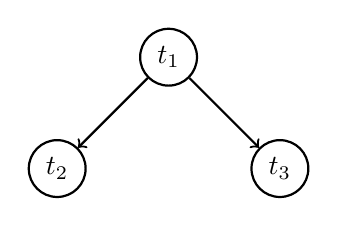
\begin{tikzpicture}[node distance={2cm}, thick, main/.style = {draw, circle}] 
        \node[main] (1) {$t_1$};
        \node[main] (2) [below left of=1] {$t_2$};
        \node[main] (3) [below right of=1] {$t_3$};

        \draw[->] (1) -- (3);
        \draw[->] (1) -- (2);

    \end{tikzpicture}
    \caption{Conflict Graph}
    \label{fig:conflict_graph_q3}
\end{figure*}\\
The equivalent serial history is $t_1t_2t_3$, and the equivalent serial schedule is \\
$s' = r_1(x) w_1(z) r_2(z) w_1(y) r_3(y) w_2(z) w_3(x) w_3(y)$. \\
As the serialization order in $s'$ is same as the actual order in $s$, hence $s \in \text{OCSR}$ also holds.

\end{document}